% Options for packages loaded elsewhere
\PassOptionsToPackage{unicode}{hyperref}
\PassOptionsToPackage{hyphens}{url}
\documentclass[
  ignorenonframetext,
]{beamer}
\newif\ifbibliography
\usepackage{pgfpages}
\setbeamertemplate{caption}[numbered]
\setbeamertemplate{caption label separator}{: }
\setbeamercolor{caption name}{fg=normal text.fg}
\beamertemplatenavigationsymbolsempty
% remove section numbering
\setbeamertemplate{part page}{
  \centering
  \begin{beamercolorbox}[sep=16pt,center]{part title}
    \usebeamerfont{part title}\insertpart\par
  \end{beamercolorbox}
}
\setbeamertemplate{section page}{
  \centering
  \begin{beamercolorbox}[sep=12pt,center]{section title}
    \usebeamerfont{section title}\insertsection\par
  \end{beamercolorbox}
}
\setbeamertemplate{subsection page}{
  \centering
  \begin{beamercolorbox}[sep=8pt,center]{subsection title}
    \usebeamerfont{subsection title}\insertsubsection\par
  \end{beamercolorbox}
}
% Prevent slide breaks in the middle of a paragraph
\widowpenalties 1 10000
\raggedbottom
\AtBeginPart{
  \frame{\partpage}
}
\AtBeginSection{
  \ifbibliography
  \else
    \frame{\sectionpage}
  \fi
}
\AtBeginSubsection{
  \frame{\subsectionpage}
}
\usepackage{iftex}
\ifPDFTeX
  \usepackage[T1]{fontenc}
  \usepackage[utf8]{inputenc}
  \usepackage{textcomp} % provide euro and other symbols
\else % if luatex or xetex
  \usepackage{unicode-math} % this also loads fontspec
  \defaultfontfeatures{Scale=MatchLowercase}
  \defaultfontfeatures[\rmfamily]{Ligatures=TeX,Scale=1}
\fi
\usepackage{lmodern}
\ifPDFTeX\else
  % xetex/luatex font selection
\fi
% Use upquote if available, for straight quotes in verbatim environments
\IfFileExists{upquote.sty}{\usepackage{upquote}}{}
\IfFileExists{microtype.sty}{% use microtype if available
  \usepackage[]{microtype}
  \UseMicrotypeSet[protrusion]{basicmath} % disable protrusion for tt fonts
}{}
\makeatletter
\@ifundefined{KOMAClassName}{% if non-KOMA class
  \IfFileExists{parskip.sty}{%
    \usepackage{parskip}
  }{% else
    \setlength{\parindent}{0pt}
    \setlength{\parskip}{6pt plus 2pt minus 1pt}}
}{% if KOMA class
  \KOMAoptions{parskip=half}}
\makeatother
\usepackage{longtable,booktabs,array}
\usepackage{caption}
\captionsetup[table]{skip=6pt}
\newcounter{none} % for unnumbered tables
\usepackage{calc} % for calculating minipage widths
\usepackage{caption}
% Make caption package work with longtable
\makeatletter
\def\fnum@table{\tablename~\thetable}
\makeatother
\usepackage{graphicx}
\makeatletter
\newsavebox\pandoc@box
\newcommand*\pandocbounded[1]{% scales image to fit in text height/width
  \sbox\pandoc@box{#1}%
  \Gscale@div\@tempa{\textheight}{\dimexpr\ht\pandoc@box+\dp\pandoc@box\relax}%
  \Gscale@div\@tempb{\linewidth}{\wd\pandoc@box}%
  \ifdim\@tempb\p@<\@tempa\p@\let\@tempa\@tempb\fi% select the smaller of both
  \ifdim\@tempa\p@<\p@\scalebox{\@tempa}{\usebox\pandoc@box}%
  \else\usebox{\pandoc@box}%
  \fi%
}
% Set default figure placement to htbp
\def\fps@figure{htbp}
\makeatother
\setlength{\emergencystretch}{3em} % prevent overfull lines
\providecommand{\tightlist}{%
  \setlength{\itemsep}{0pt}\setlength{\parskip}{0pt}}
% Auto-generated by infrastructure/rendering/_pdf_latex_helpers.py::extract_math_font_preamble.
% Minimal header passed to Pandoc via -H so Beamer slides pick up the same math font
% as the combined-PDF path. Adjust the manuscript's preamble.md to change the font globally.
\usepackage{unicode-math}
\setmathfont{latinmodern-math.otf}

% Slide layout defaults for warning-clean scientific decks.
\usepackage{etoolbox}
\IfFileExists{xurl.sty}{\usepackage{xurl}}{}
\IfFileExists{seqsplit.sty}{\usepackage{seqsplit}}{\newcommand{\seqsplit}[1]{#1}}
\protected\def\breakseq#1{\seqsplit{#1}}
\protected\def\breaktt#1{\begingroup\ttfamily\seqsplit{#1}\endgroup}
\setlength{\emergencystretch}{6em}
\tolerance=5000
\hbadness=10000
\hfuzz=1pt
\setlength{\tabcolsep}{2pt}
\AtBeginEnvironment{longtable}{\tiny\renewcommand{\arraystretch}{0.86}\setlength{\tabcolsep}{1pt}}
\AtBeginEnvironment{tabular}{\tiny\renewcommand{\arraystretch}{0.86}\setlength{\tabcolsep}{1pt}}
\AtBeginEnvironment{equation}{\tiny}
\AtBeginEnvironment{equation*}{\tiny}
\AtBeginEnvironment{align}{\tiny}
\AtBeginEnvironment{align*}{\tiny}
\AtBeginEnvironment{itemize}{\footnotesize}
\AtBeginEnvironment{enumerate}{\footnotesize}
\AtBeginEnvironment{description}{\footnotesize}
\setbeamerfont{caption}{size=\tiny}
\setbeamerfont{caption name}{size=\tiny}
\setbeamerfont{normal text}{size=\small}
\setbeamerfont{frametitle}{size=\small}
\setbeamerfont{section title}{size=\footnotesize}
\setbeamerfont{subsection title}{size=\footnotesize}
\setbeamertemplate{section page}{%
  \centering
  \begin{beamercolorbox}[sep=12pt,center,wd=\paperwidth]{section title}
    \parbox{0.86\paperwidth}{\centering\usebeamerfont{section title}\insertsection\par}
  \end{beamercolorbox}
}
\setbeamertemplate{subsection page}{%
  \centering
  \begin{beamercolorbox}[sep=8pt,center,wd=\paperwidth]{subsection title}
    \parbox{0.86\paperwidth}{\centering\usebeamerfont{subsection title}\insertsubsection\par}
  \end{beamercolorbox}
}
\setlength{\abovecaptionskip}{2pt}
\setlength{\belowcaptionskip}{0pt}

% Natbib and cross-reference fallbacks — slides don't load natbib
% or cleveref, but combined-PDF manuscript prose may emit these
% commands. The fallback renders citations as a bracketed key list
% and cross-references as detokenized labels so slides don't fail on
% undefined control sequences or raw underscores. \providecommand is
% a no-op if packages load later.
\providecommand{\citep}[1]{[#1]}
\providecommand{\citet}[1]{#1}
\providecommand{\citealp}[1]{#1}
\providecommand{\citeauthor}[1]{#1}
\providecommand{\citeyear}[1]{#1}
\providecommand{\cref}[1]{\texttt{\detokenize{#1}}}
\providecommand{\Cref}[1]{\texttt{\detokenize{#1}}}

\newtheorem{proposition}{Proposition}
\newtheorem{hypothesis}{Hypothesis}
\usepackage{bookmark}
\IfFileExists{xurl.sty}{\usepackage{xurl}}{} % add URL line breaks if available
\urlstyle{same}
% fallback for those not using the hyperref driver hyperxmp:
\makeatletter
\@ifundefined{xmpquote}{\newcommand{\xmpquote}[1]{#1}}{}
\makeatother
\hypersetup{
  hidelinks,
  pdfcreator={LaTeX via pandoc}}

\author{\texorpdfstring{}{}}
\date{}

\begin{document}

\section{Results: SkillTree Export and Learner-Surface
Handoff}\label{sec:results-skilltree-dashboard-front-matter}

\begin{frame}[fragile,allowframebreaks]{SkillTree export,
learner-surface handoff, and generated front matter}
\protect\phantomsection\label{skilltree-export-learner-surface-handoff-and-generated-front-matter}
All registered claims are produced by tested kernels; every claim token
in the 630 skills resolves, and the bare-number linter reports zero
violations across descriptions, assessment prompts, and correct numeric
answer options. The scholarship audit similarly resolves every authored
citation against the bibliography and source-role matrix. The
provenance-rendered graph exports to a SkillTree project of 111
subjects, 630 skills, 1199 learning-path dependencies, 630 quizzes, and
2520 assessment questions, with no unresolved tokens in the output. The
source reaches the configured \texttt{src/} coverage gate with no mocks;
exact current coverage is reported by the test run rather than asserted
in prose.

\end{frame}

\begin{frame}[fragile,allowframebreaks]{SkillTree export,
learner-surface handoff, and generated front matter}
The dashboard delivery surface exposes the same contract. Its status
payload cross-checks SkillTree export counts against build stats, tracks
the claim ledger and figure artifacts, exposes the manuscript artifact
audit, mounts the official learner display when SkillTree is online, and
gives each skill a direct handoff into that display's subject and
quiz-gated skill pages. This avoids the common false demo in which a
polished local UI merely copies course text: the local page can inspect
and preview artifacts, but the learning and quiz actions are routed to
the seeded SkillTree project.

\end{frame}

\begin{frame}[fragile,allowframebreaks]{SkillTree export,
learner-surface handoff, and generated front matter}
Prose cannot settle that distinction, so the delivery surface is also
recorded directly. fig.~\ref{fig:app_operational_snapshot} shows the
landing view reporting exported counts, live SkillTree dependency
parity, and artifact presence together.
fig.~\ref{fig:app_official_learner_view} shows SkillTree's own client
library rendering the seeded project inside the local page, with its
native points, level, progress rings, and ranking; that is the
observation the export-lands-in-the-platform reading needs, and no
exported JSON file can supply it.
fig.~\ref{fig:app_curriculum_learn_material} shows the generated lesson
record for one skill beside its commit-pinned upstream pointers, so the
material boundary is visible rather than asserted.
fig.~\ref{fig:app_dependency_graph} shows the captioned
prerequisite-flow table that carries the heaviest subject-to-subject
relations for readers who cannot use the lane drawing, which is a ranked
\end{frame}

\begin{frame}[fragile,allowframebreaks]{SkillTree export,
learner-surface handoff, and generated front matter}
summary of that structure rather than a complete substitute for every
edge, and fig.~\ref{fig:app_runtime_deployment_matrix} shows
deployment-mode readiness beside the browser-visible runtime payload,
where the admin password and client secret are absent. These five images
are recordings rather than renders: unlike every other figure here they
cannot be rebuilt from project data, so they are version-controlled,
marked in the figure registry as captured evidence, and stamped with the
dashboard URL, viewport, live counts, capture timestamp, per-image
digest, and full-stack mode of the run that produced them. Being
recordings, they are also the one family exempt from the check that
every registered figure was emitted by the render pipeline; the
exemption is recorded in the registry rather than left implicit, and
their integrity rests on the digest and provenance record instead.

\end{frame}

\begin{frame}[fragile,allowframebreaks]{SkillTree export,
learner-surface handoff, and generated front matter}
The front matter follows the same rule. The cover image is generated
from the live graph, claim registry and roadmap metrics, and the
page-two named-skill atlas is generated from every authored skill name
in the curriculum graph. Both images are checked by publication-asset
audits before rendering. The cover uses a square layout so it can serve
both PDF title-page and web artifact contexts; the atlas uses a wide
page-two layout so the skill-name vocabulary remains readable by showing
a reduced weighted-term sample and representative dependency checkpoints
rather than a complete printed index. Neither asset is a numbered
scientific figure: the dashboard exposes them as cover-category
artifacts, while \breaktt{figure\_registry.json} remains reserved for
manuscript figures that are declared and cross-referenced in the text.
This prevents polished front matter from becoming a false-certification
\end{frame}

\begin{frame}[fragile,allowframebreaks]{SkillTree export,
learner-surface handoff, and generated front matter}
path outside the artifact contract.

\end{frame}

\begin{frame}[fragile,allowframebreaks]{SkillTree export,
learner-surface handoff, and generated front matter}
\begin{figure}
\centering
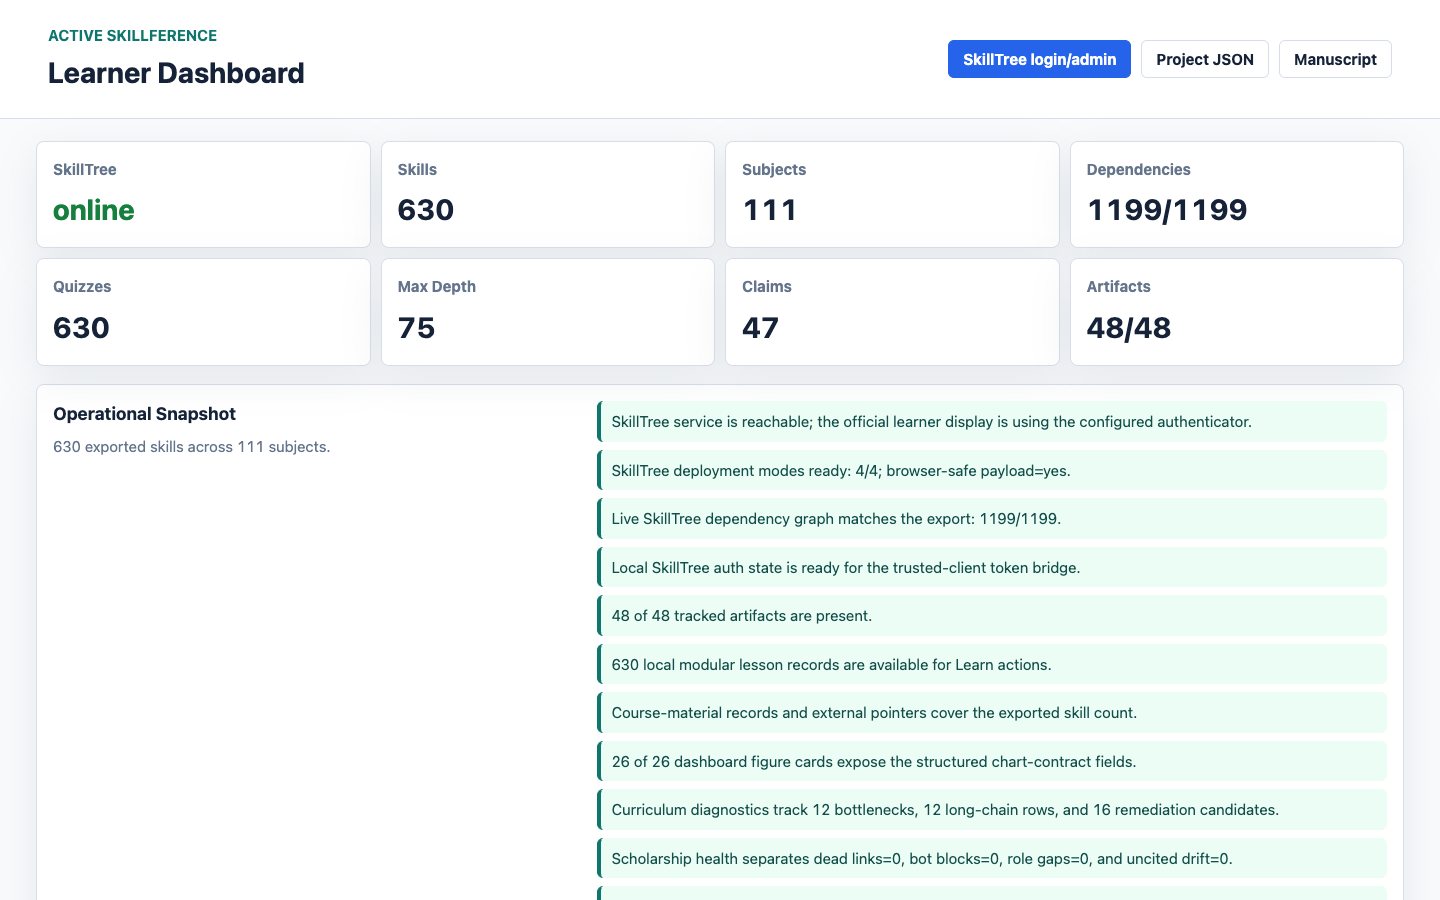
\includegraphics[width=1\linewidth,height=0.40\textheight,keepaspectratio,alt={Learner dashboard landing view captured from the running local stack. The metric row reports exported skills, subjects, quizzes, maximum prerequisite depth, registered claims, and artifact presence, while the dependency metric shows live SkillTree parity against the export rather than the exported count alone. The evidence list below restates those machine-checked conditions in words: export counts, live graph parity, local auth readiness, course-material coverage, and figure-contract completeness are surfaced together on one page instead of being scattered across separate reports. The list continues past the fold; the frame shows the first ten of its rows. The artifact tally counts this evidence family among the tracked artifacts, so it is a completeness check on the roster rather than an independent audit of these images.}]{../figures/app_operational_snapshot.png}
\caption{Learner dashboard landing view captured from the running local
stack. The metric row reports exported skills, subjects, quizzes,
maximum prerequisite depth, registered claims, and artifact presence,
while the dependency metric shows live SkillTree parity against the
export rather than the exported count alone. The evidence list below
restates those machine-checked conditions in words: export counts, live
graph parity, local auth readiness, course-material coverage, and
figure-contract completeness are surfaced together on one page instead
of being scattered across separate reports. The list continues past the
fold; the frame shows the first ten of its rows. The artifact tally
counts this evidence family among the tracked artifacts, so it is a
completeness check on the roster rather than an independent audit of
these images.}\label{fig:app_operational_snapshot}
\end{figure}

\begin{figure}
\centering
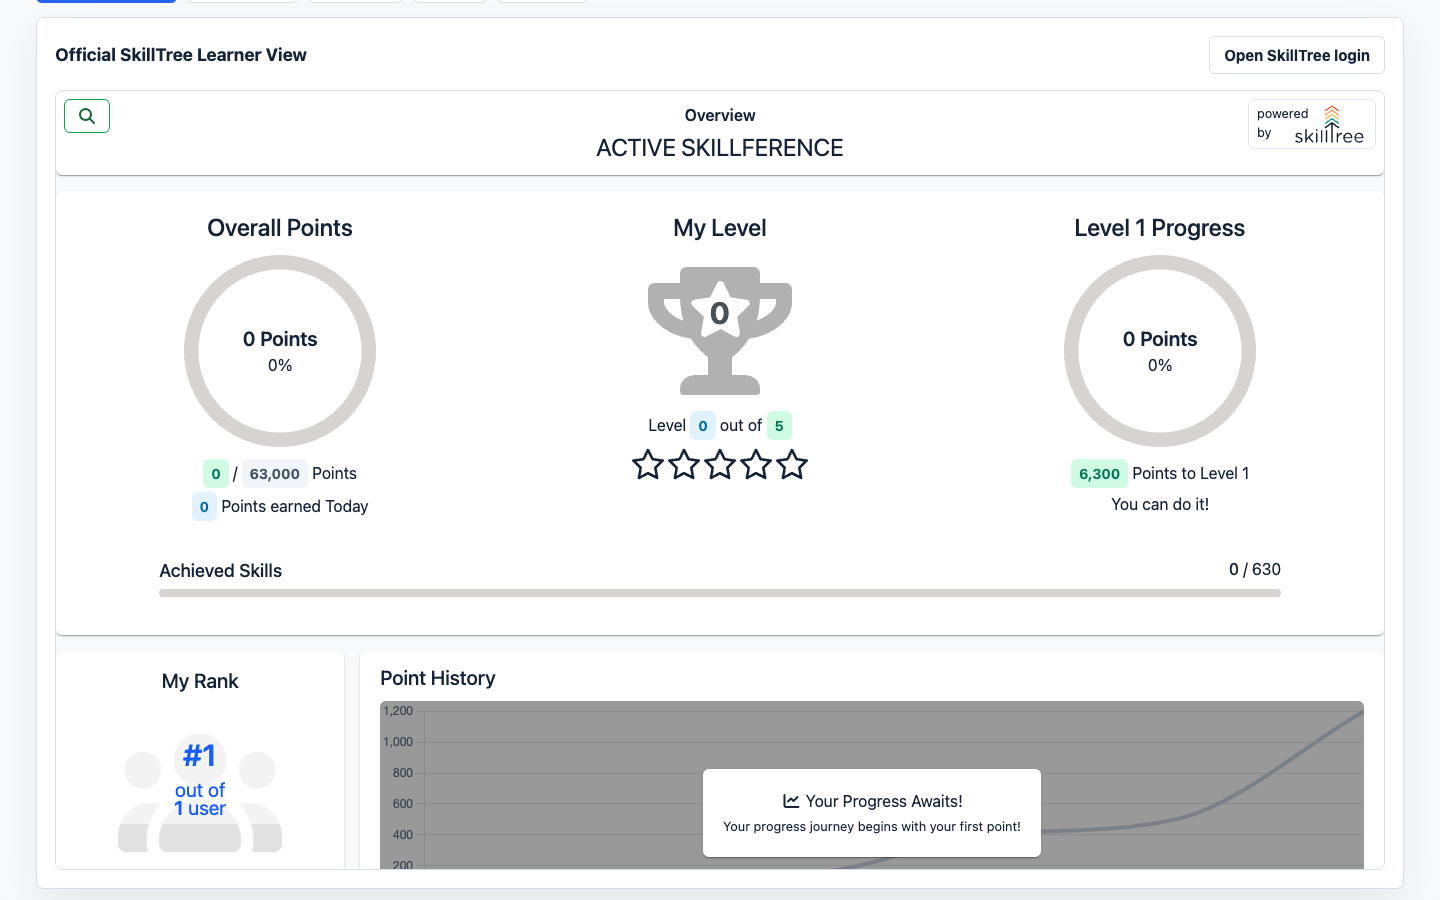
\includegraphics[width=1\linewidth,height=0.40\textheight,keepaspectratio,alt={The Official Display tab captured while the embedded SkillTree learner client is mounted against the seeded project. The overview header, overall points, level and level progress rings, the achieved-skills bar reading zero of the full exported skill count, the personal rank card, and the point-history panel are all rendered by SkillTree's own client library inside the project dashboard, which is the demonstration that the export lands in the platform runtime rather than in a project reimplementation of it. Every progress value reads zero and the point-history panel shows its first-point empty state, because the capture uses a freshly seeded local identity that has completed nothing.}]{../figures/app_official_learner_view.png}
\caption{The Official Display tab captured while the embedded SkillTree
learner client is mounted against the seeded project. The overview
header, overall points, level and level progress rings, the
achieved-skills bar reading zero of the full exported skill count, the
personal rank card, and the point-history panel are all rendered by
SkillTree's own client library inside the project dashboard, which is
the demonstration that the export lands in the platform runtime rather
than in a project reimplementation of it. Every progress value reads
zero and the point-history panel shows its first-point empty state,
because the capture uses a freshly seeded local identity that has
completed nothing.}\label{fig:app_official_learner_view}
\end{figure}

\begin{figure}
\centering
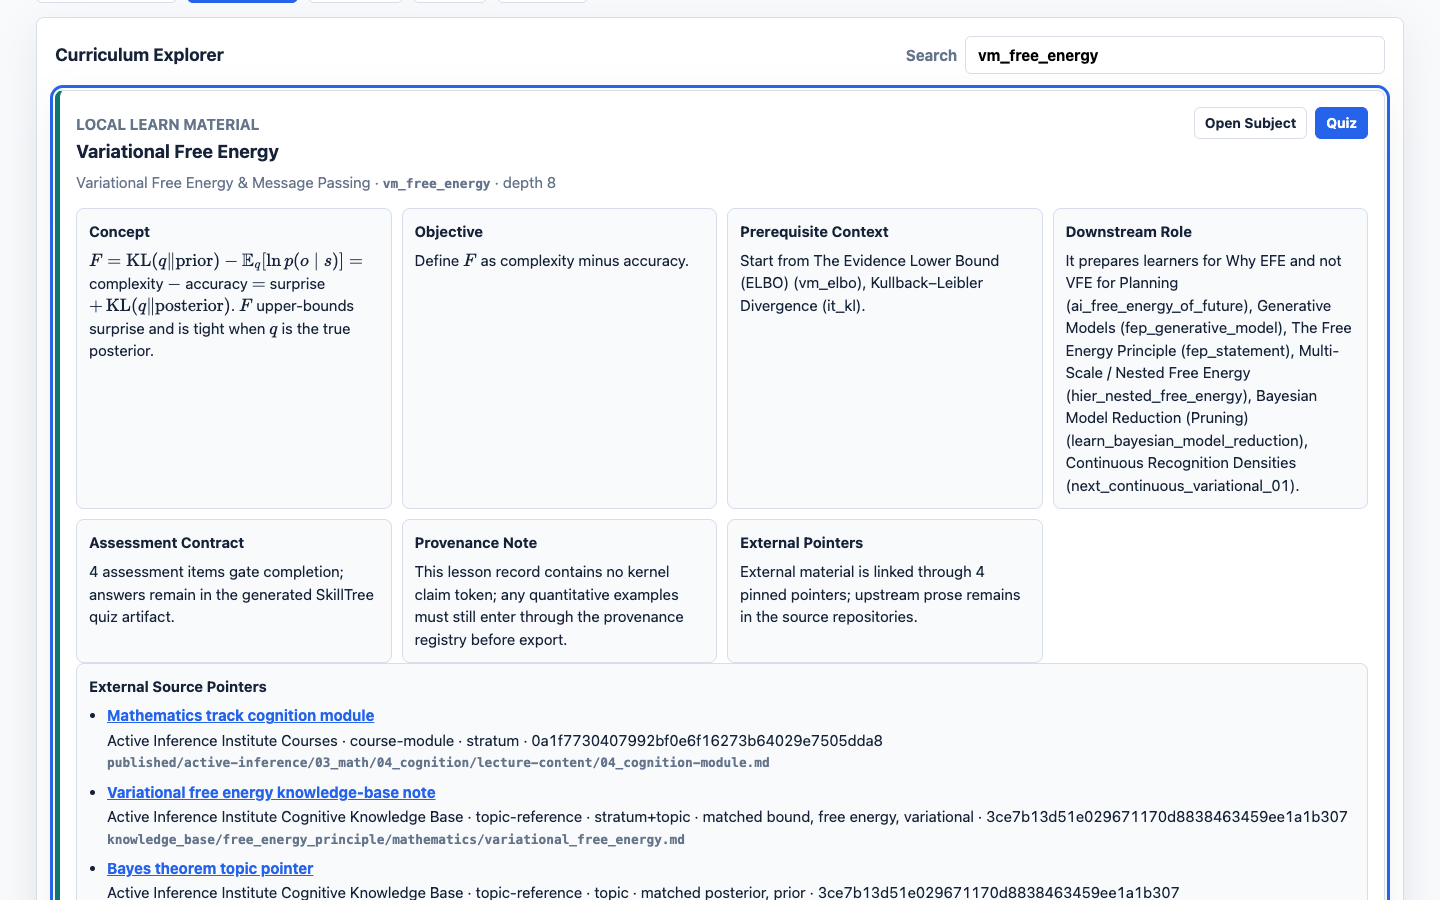
\includegraphics[width=1\linewidth,height=0.40\textheight,keepaspectratio,alt={The Curriculum tab captured with the generated lesson record for the variational free energy skill opened through its Learn action. The panel shows the concept context, prerequisite position, downstream role, assessment summary, and the commit-pinned external source pointers generated for that skill, alongside the handoff buttons that return the learner to the official SkillTree subject and quiz routes. It is the delivery counterpart to the course-material provenance rule: local lessons link out to pinned upstream sources instead of copying them.}]{../figures/app_curriculum_learn_material.png}
\caption{The Curriculum tab captured with the generated lesson record
for the variational free energy skill opened through its Learn action.
The panel shows the concept context, prerequisite position, downstream
role, assessment summary, and the commit-pinned external source pointers
generated for that skill, alongside the handoff buttons that return the
learner to the official SkillTree subject and quiz routes. It is the
delivery counterpart to the course-material provenance rule: local
lessons link out to pinned upstream sources instead of copying
them.}\label{fig:app_curriculum_learn_material}
\end{figure}

\begin{figure}
\centering
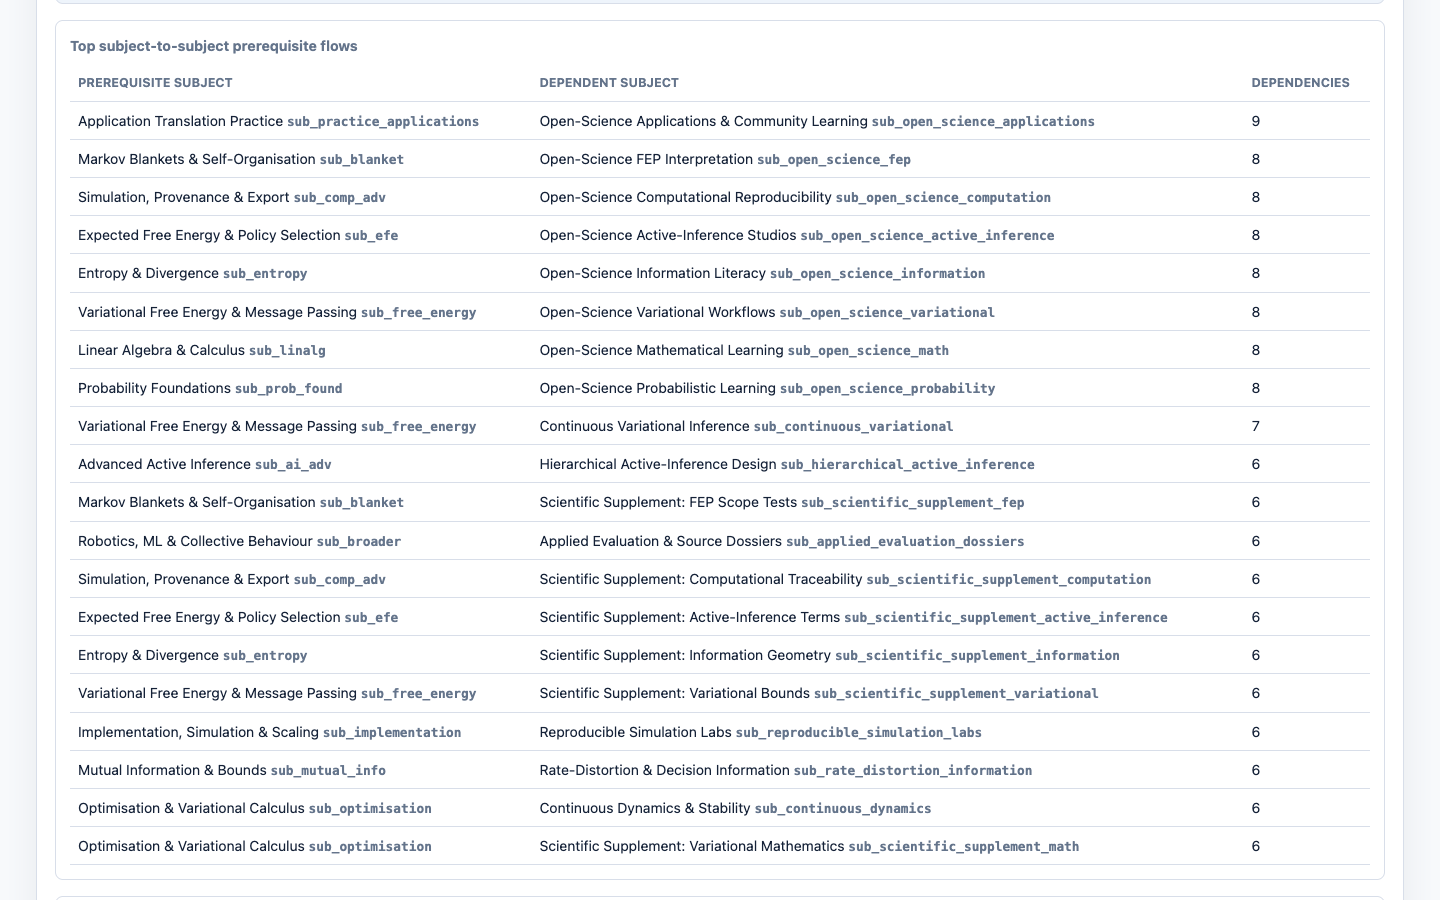
\includegraphics[width=1\linewidth,height=0.40\textheight,keepaspectratio,alt={The accessible prerequisite-flow table in the Graph tab, scrolled past the subject lane canvas that sits above it in the same panel. Table and canvas are built from the same server-computed flow summaries, so the prerequisite structure reaches a keyboard or screen-reader user as captioned rows with real header cells rather than only as a drawing. Each row is one directed subject-to-subject relation: a prerequisite subject, the dependent subject that requires it, and how many skill dependencies run between them, ordered by weight.}]{../figures/app_dependency_graph.png}
\caption{The accessible prerequisite-flow table in the Graph tab,
scrolled past the subject lane canvas that sits above it in the same
panel. Table and canvas are built from the same server-computed flow
summaries, so the prerequisite structure reaches a keyboard or
screen-reader user as captioned rows with real header cells rather than
only as a drawing. Each row is one directed subject-to-subject relation:
a prerequisite subject, the dependent subject that requires it, and how
many skill dependencies run between them, ordered by
weight.}\label{fig:app_dependency_graph}
\end{figure}

\begin{figure}
\centering
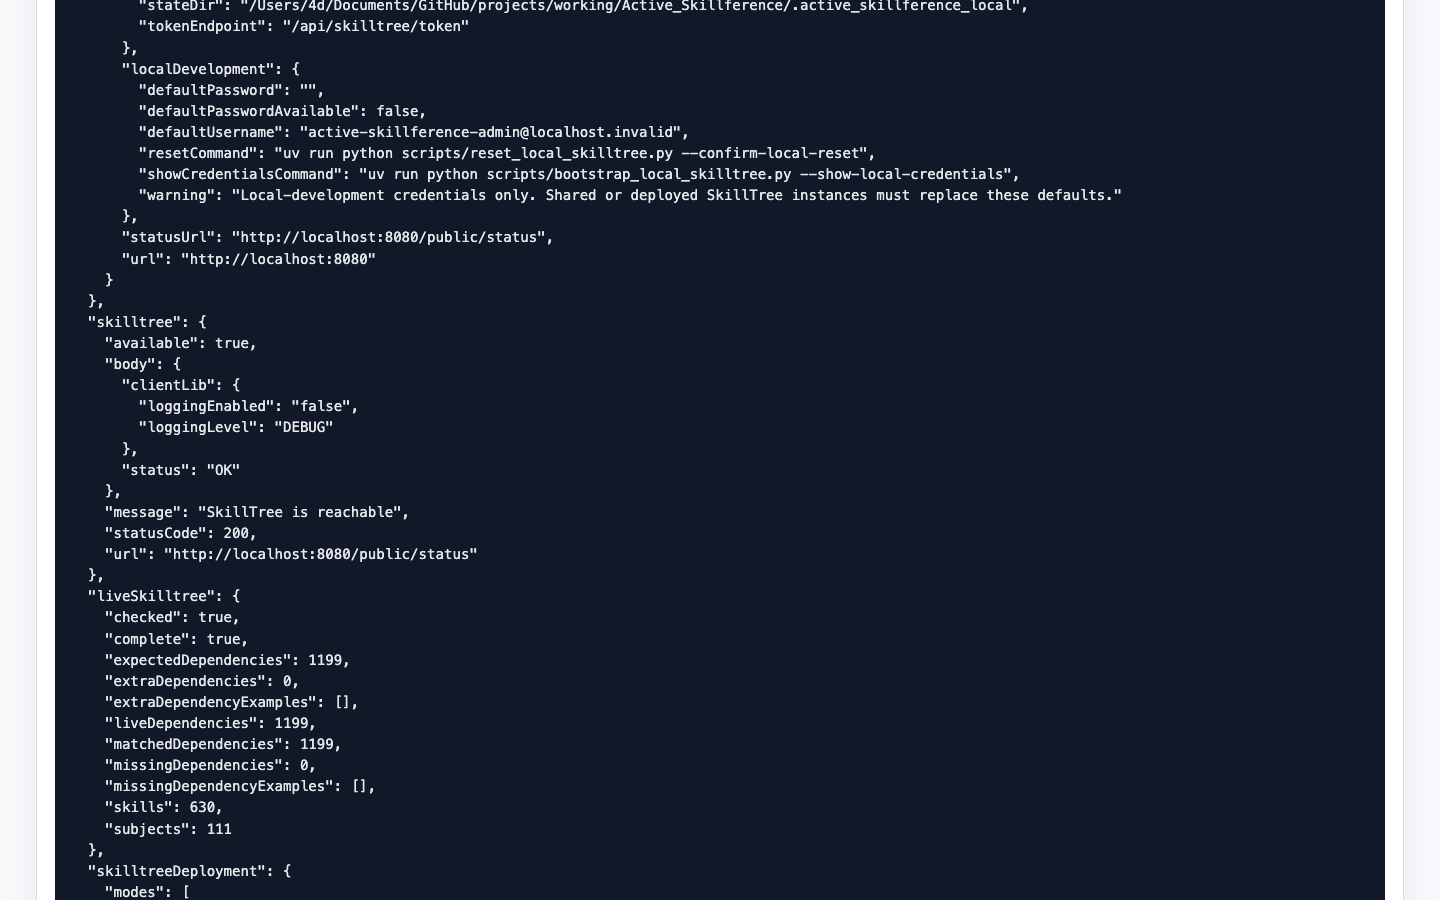
\includegraphics[width=1\linewidth,height=0.40\textheight,keepaspectratio,alt={The browser-visible runtime payload in the Runtime tab, scrolled past the deployment-mode matrix to the local development block. The default password field is an empty string and its availability flag is false, so the page reports the local username and the recovery commands while withholding the credential itself; no client secret and no bearer token appear anywhere in the payload. The same view carries the SkillTree reachability block and the live dependency parity block reporting complete parity with no missing or extra edges, which is the auth-boundary evidence in the form the browser actually receives it.}]{../figures/app_runtime_deployment_matrix.png}
\caption{The browser-visible runtime payload in the Runtime tab,
scrolled past the deployment-mode matrix to the local development block.
The default password field is an empty string and its availability flag
is false, so the page reports the local username and the recovery
commands while withholding the credential itself; no client secret and
no bearer token appear anywhere in the payload. The same view carries
the SkillTree reachability block and the live dependency parity block
reporting complete parity with no missing or extra edges, which is the
auth-boundary evidence in the form the browser actually receives
it.}\label{fig:app_runtime_deployment_matrix}
\end{figure}
\end{frame}

\end{document}
